\documentclass[14pt, fleqn, xcolor={dvipsnames, table}]{beamer}
\usepackage[T2A]{fontenc}
\usepackage[utf8]{inputenc}
\usepackage[english,russian]{babel}
\usepackage{amssymb,amsfonts,amsmath,mathtext}
\usepackage{cite,enumerate,float,indentfirst}
\usepackage{cancel}

\usepackage{tikz}                   
\usetikzlibrary{shadows}

% \usepackage{enumitem}
% \setitemize{label=\usebeamerfont*{itemize item}%
%   \usebeamercolor[fg]{itemize item}
%   \usebeamertemplate{itemize item}}

\graphicspath{{images/}}

\usetheme{Madrid}
\usecolortheme{seahorse}
\renewcommand{\CancelColor}{\color{red}}

\setbeamercolor{footline}{fg=Blue!50}
\setbeamertemplate{footline}{
  \leavevmode%
  \hbox{%
  \begin{beamercolorbox}[wd=.333333\paperwidth,ht=2.25ex,dp=1ex,center]{}%
    И. Кураленок, Н. Поваров, Яндекс
  \end{beamercolorbox}%
  \begin{beamercolorbox}[wd=.333333\paperwidth,ht=2.25ex,dp=1ex,center]{}%
    Санкт-Петербург, 2013
  \end{beamercolorbox}%
  \begin{beamercolorbox}[wd=.333333\paperwidth,ht=2.25ex,dp=1ex,right]{}%
  Стр. \insertframenumber{} из \inserttotalframenumber \hspace*{2ex}
  \end{beamercolorbox}}%
  \vskip0pt%
}
\newcommand\indentdisplays[1]{%
     \everydisplay{\addtolength\displayindent{#1}%
     \addtolength\displaywidth{-#1}}}
\newcommand{\itemi}{\item[\checkmark]}

\title{Линейные модели: уменьшаем variance\\\small{}}
\author[]{\small{%
И.~Куралёнок,
Н.~Поваров}}
\date{}

\begin{document}

\begin{frame}
\maketitle
\small
\begin{center}
\vspace{-60pt}
\normalsize {\color{red}Я}ндекс \\
\vspace{80pt}
\footnotesize СПб, 2013
\end{center}
\end{frame}

\section{Постановка задачи восстановления сигнала}
\subsection{Пример}
\subsection{Разложение сигнала в Фурье и постановка в нахождении коэффициентов}
\section{LASSO для восстановления сигнала}
\subsection{Теорема о качестве восстановленного сигнала (Candes et al. 2006)}
\subsection{Стабильность решения: RIP, RRfND (Candes et al. 2006)}
\subsection{LASSO persistency theorem (Bickel et al., 2009)}
\section{Support vector machines}
\subsection{Идея метода}
\begin{frame}{SVM(воспоминания о былом)}
\begin{itemize}
  \item Последний из линейных методов, который мы рассмотрим подробно.
  \item Rocket science до конца 90-х, по крайней мере в задачах классификации.
\end{itemize}
\end{frame}

\begin{frame}{SVM на пальцах}
\begin{itemize}
  \item Максимальный зазор.
  \item Нелинейные преобразования.
\end{itemize}
\begin{center}
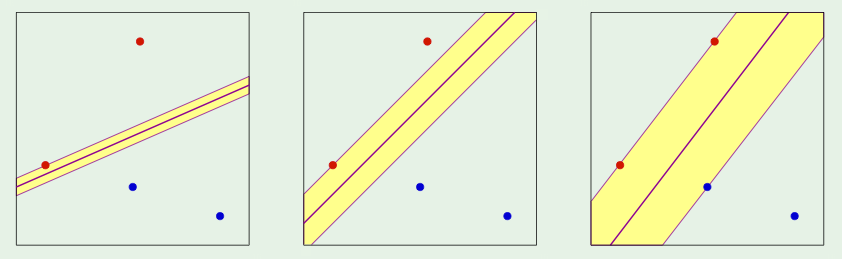
\includegraphics[width=0.9\textwidth]{SVM_1.png}
\end{center}
\end{frame}

\begin{frame}{Мысли вслух}
\begin{itemize}
  \item Почему большой зазор это хорошо?
  \item Какая $\beta$ максимизирует зазор? 
\end{itemize}
\end{frame}

\subsection{Коэффициенты Лагранжа для решения задачи про максимальное расстояние}
\subsection{Переход к дуальному решению}
\subsection{Идея как можно на халяву это решить}
\subsection{Kernel trick}
\subsection{Сведение SVM к регуляризации (основная идея)}
\subsection{Домашнее задание}
\begin{frame}{Результаты ДЗ четвёртой недели}
\tiny
\begin{center}
\begin{enumerate}
\item ca876
\item 3fc89
\item e46c8
\item 76a61
\item 165f4
\item 729da
\item cd90b
\item cdb5c
\item 23449
\item c8b18
\item 5660e
\item 257d3
\item 2431e
\item 346a9
\item 6f1ba
\item ab851
\item 3ebe0
\item 49dd1
\item 1938b
\end{enumerate}
\end{center}
\end{frame}

\begin{frame}{Интерпретация результатов}
Задача была придумать несколько таргетов.
\begin{center}
\begin{itemize}
\item 1 место - очень круто;
\item 2 место - почти очень круто;
\item 3-4 места - знают, что такое целевая функция, помнят про "бесконечные потери";
\item 5-10 места - знают, что такое целевая функция, но местами забыли про "бесконечные потери";
\item 11-12 места - знают, что такое целевая функция, но забыли про "бесконечные потери" совсем;
\item 13-19 места - перепутали целевую функцию с решающей, а особо отличившиеся с факторами.
\end{itemize}
\end{center}
\end{frame}

\begin{frame}{Домашнее задание}
\begin{itemize}
\item датасет тот же;
\item сегодня узнали про новые методы - будем применять;
\item howto.txt;
\item дедлайн - 29 ноября.
\end{itemize}
\end{frame}

\end{document}
